\chapter{Analysephase}
\label{chap:analysephase}

Die Anforderungen an das geplante Tool wurden auf Basis von Stakeholder-Interviews und einer Analyse bestehender Lösungen definiert. Ziel war es, eine effektive, skalierbare und benutzerfreundliche Lösung zu entwerfen, die den spezifischen Anforderungen von Führungskräften und HR-Managern entspricht.

\section{Anforderungen}
Um die Funktionalität und Effizienz des Systems sicherzustellen, wurden sowohl funktionale als auch nicht-funktionale Anforderungen formuliert. Die funktionalen Anforderungen umfassen Kernfunktionen wie interaktive Visualisierungen, Datenmanagement und Benutzerverwaltung, während nicht-funktionale Anforderungen Aspekte wie Sicherheit, Performance und Skalierbarkeit adressieren.

Das System soll die Visualisierung von Daten durch interaktive Donut- und Radarcharts ermöglichen, um Trends und Leistungskennzahlen übersichtlich darzustellen \cite{kirk2016data}. Gleichzeitig soll ein strukturiertes Datenmanagement den Import, die Speicherung und die Bearbeitung von Gesprächsdaten sicherstellen, um Nachverfolgbarkeit und Konsistenz zu gewährleisten \cite{bryson2011employee}. Zusätzlich wird ein Exportmodul benötigt, um Berichte in Formaten wie Excel und PDF für weiterführende Analysen bereitzustellen. Die Benutzerverwaltung des Tools ermöglicht differenzierte Zugriffskontrollen, die sensible Daten schützen und rollenbasierten Zugriff gewährleisten \cite{duarte2012performance}.

Nicht-funktionale Anforderungen konzentrieren sich auf die Qualität des Tools. Die Performance des Systems muss auch bei großen Datenmengen eine schnelle Verarbeitung gewährleisten. Die Skalierbarkeit soll sicherstellen, dass das System mit wachsender Nutzer- und Datenanzahl effizient arbeitet. Zudem ist die Sicherheit durch moderne Authentifizierungs- und Verschlüsselungsmethoden zu gewährleisten, um sensible Informationen zu schützen \cite{schober2008}.

\section{Stakeholder-Interviews und Umfragen}
Zur Ermittlung der Anforderungen wurden zwischen März und Mai 2024 halbstrukturierte Interviews mit 15 Führungskräften und HR-Managern aus verschiedenen Abteilungen des Unternehmens durchgeführt. Die Teilnehmenden wurden gezielt ausgewählt, um unterschiedliche Perspektiven und Anforderungen abzudecken, darunter Vertreter aus operativen und strategischen Bereichen. Die Gespräche dauerten durchschnittlich 45 Minuten und umfassten Themen wie relevante Daten für Entscheidungsfindungen, Herausforderungen bestehender Tools und essenzielle Funktionen für die tägliche Arbeit.

Die Antworten wurden qualitativ analysiert, um zentrale Anforderungen und Prioritäten zu identifizieren. Die Ergebnisse zeigten, dass Datensicherheit und benutzerfreundliche Visualisierungen höchste Priorität hatten. Darüber hinaus bestand der Wunsch nach einer dynamischen Benutzeroberfläche mit Echtzeit-Updates.

\subsection{Ergebnisse}
Die Analyse der Interviews ergab folgende zentrale Anforderungen:
\begin{itemize}
    \item \textbf{Intuitive Diagramme:} Visualisierungen, die Trends und Muster schnell erkennbar machen.
    \item \textbf{Echtzeit-Updates:} Dynamische Benutzeroberfläche mit aktuellen Daten.
    \item \textbf{Datensicherheit:} Strikte Anforderungen an den Schutz sensibler Gesprächsdaten \cite{bryson2011employee}.
\end{itemize}

\begin{figure}[h!]
    \centering
    Die Abbildung illustriert die Häufigkeit, mit der 32 Mitarbeiter bestimmte Anforderungen während der Stakeholder-Interviews genannt haben. Dabei zeigt sich, dass Datensicherheit die höchste Priorität hatte, gefolgt von der Nachfrage nach Visualisierungen und Echtzeit-Updates. Diese Ergebnisse verdeutlichen die zentralen Schwerpunkte, die bei der Entwicklung des Tools berücksichtigt werden sollten.
    
    % Abbildung
    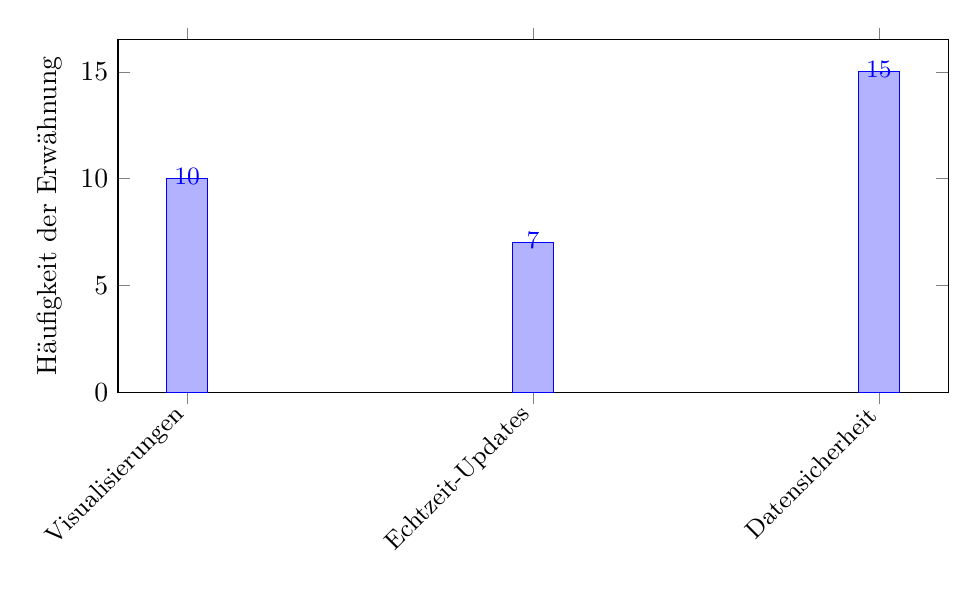
\begin{tikzpicture}
        \begin{axis}[
            width=\textwidth,
            height=0.5\textwidth,
            ybar,
            bar width=15pt,
            ylabel={Häufigkeit der Erwähnung},
            symbolic x coords={Visualisierungen, Echtzeit-Updates, Datensicherheit},
            xtick=data,
            x tick label style={font=\small, rotate=45, anchor=east},
            ymin=0,
            nodes near coords,
            nodes near coords style={font=\small, anchor=mid},
        ]
        \addplot coordinates {(Visualisierungen,10) (Echtzeit-Updates,7) (Datensicherheit,15)};
        \end{axis}
    \end{tikzpicture}
    \caption{Häufigkeit genannter Anforderungen aus Stakeholder-Interviews.}
    \label{fig:stakeholder_results_barchart}
\end{figure}

\section{Einordnung bestehender Lösungen}
Zur Bewertung der vorhandenen Marktsituation wurden die Tools HRworks und Evalea analysiert, die als etablierte Lösungen im HR-Bereich gelten. Beide Systeme bieten spezifische Funktionen zur Unterstützung von HR-Prozessen, weisen jedoch Einschränkungen in der Visualisierung von Daten und der Anpassungsfähigkeit an unternehmensspezifische Anforderungen auf.

HRworks fokussiert sich auf die allgemeine Verwaltung von HR-Daten und bietet Basisfunktionen wie eine intuitive Benutzeroberfläche und 360°-Feedback-Optionen. Evalea hingegen punktet durch umfangreichere Reporting-Funktionen und anpassbare Gesprächsleitfäden. Beide Tools bieten jedoch keine interaktiven Visualisierungsmöglichkeiten, wie sie für das geplante System vorgesehen sind. Im Vergleich zu den Anforderungen des geplanten Tools wird deutlich, dass insbesondere die Echtzeit-Visualisierung und die tiefergehende Integration in bestehende Systeme fehlen.

\begin{figure}[h!]
    \centering
    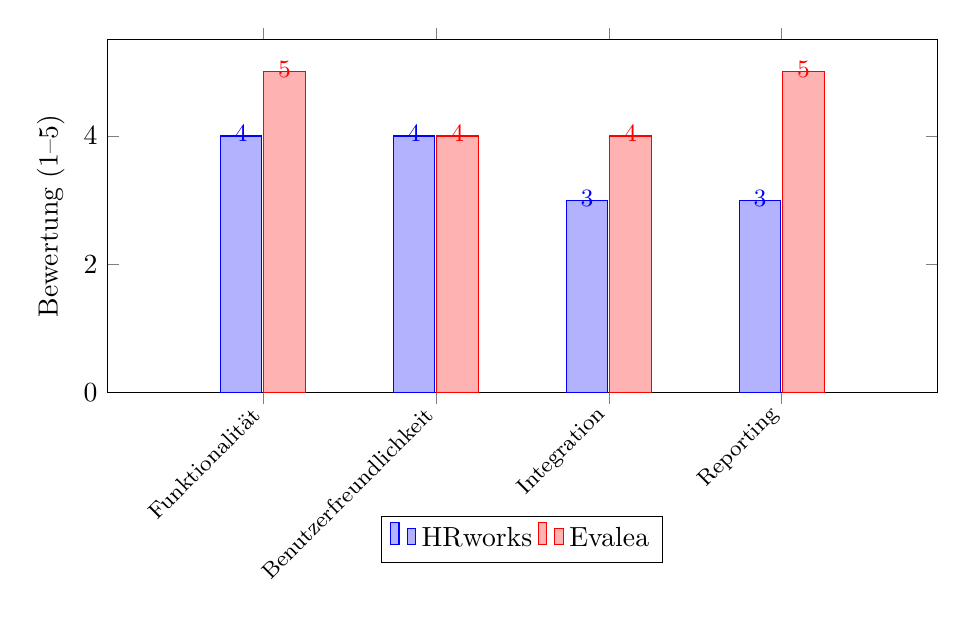
\begin{tikzpicture}
        \begin{axis}[
            width=\textwidth,
            height=0.5\textwidth,
            ybar=0.7pt,
            bar width=15pt,
            enlarge x limits=0.3,
            ylabel={Bewertung (1–5)},
            symbolic x coords={Funktionalität, Benutzerfreundlichkeit, Integration, Reporting},
            xtick=data,
            x tick label style={font=\footnotesize, rotate=45, anchor=east},
            ymin=0, ymax=5.5,
            nodes near coords,
            nodes near coords style={font=\small, anchor=mid},
            legend style={at={(0.5,-0.35)}, anchor=north, legend columns=-1},
            legend cell align={left}
        ]
        \addplot[blue,fill=blue!30] coordinates {
            (Funktionalität,4)
            (Benutzerfreundlichkeit,4)
            (Integration,3)
            (Reporting,3)
        };
        \addplot[red,fill=red!30] coordinates {
            (Funktionalität,5)
            (Benutzerfreundlichkeit,4)
            (Integration,4)
            (Reporting,5)
        };
        \legend{HRworks, Evalea}
        \end{axis}
    \end{tikzpicture}
    \caption{Vergleich zwischen HRworks und Evalea in verschiedenen Kategorien.}
    \label{fig:hrworks_evalea_comparison}
\end{figure}

\section{Zusammenfassung}
Die Analysephase verdeutlichte, dass das geplante System eine klare Lücke in den bestehenden HR-Tools schließen kann. Die Anforderungen aus den Stakeholder-Interviews sowie die Evaluation bestehender Lösungen bilden die Grundlage für die Entwicklung eines Systems, das durch benutzerfreundliche Visualisierungen, Sicherheit und Skalierbarkeit überzeugt. Dies ermöglicht eine effektive Unterstützung von HR-Abteilungen bei datenbasierten Entscheidungen und der strategischen Planung.

